\documentclass[11pt,border=2pt]{standalone}
\usepackage{tikz}
\usetikzlibrary{arrows.meta,positioning,calc,fit,backgrounds,shapes.geometric}
\usepackage{amsmath,amssymb}
\usepackage{times}
\definecolor{ink}{HTML}{243447}
\definecolor{cA}{HTML}{4477AA}
\definecolor{cB}{HTML}{CC6677}
\definecolor{cAu}{HTML}{44AA99}
\definecolor{cS}{HTML}{CCAA33}
\definecolor{grn}{HTML}{228833}
\definecolor{rose}{HTML}{AA3377}
\definecolor{inst}{HTML}{F2E3B3}
\tikzset{
 pap/.style={circle,draw=ink,line width=.6pt,minimum size=15pt,inner sep=0pt,font=\scriptsize\bfseries,text=white},
 aut/.style={rectangle,draw=ink,line width=.6pt,minimum size=13pt,inner sep=0pt,fill=cAu,font=\scriptsize\bfseries,text=white},
 sub/.style={diamond,draw=ink,line width=.6pt,minimum size=17pt,inner sep=0pt,fill=cS,font=\scriptsize\bfseries,text=white},
 gone/.style={draw=ink!35,fill=ink!8,text=ink!40,dashed},
 ed/.style={draw=ink,line width=.7pt},
 msg/.style={-{Stealth[length=4pt]},line width=.9pt,draw=rose},
 ptitle/.style={font=\footnotesize\bfseries,text=ink,anchor=west},
 note/.style={font=\scriptsize,text=ink,align=center},
}

\definecolor{fcF}{HTML}{AA3377}
\definecolor{fcG}{HTML}{EE7733}
\definecolor{lrn}{HTML}{CC3311}
\definecolor{rel}{HTML}{6A51A3}
\tikzset{
 pap/.style={circle,draw=ink,line width=.7pt,minimum size=19pt,inner sep=0pt,font=\footnotesize\bfseries,text=white},
 aut/.style={rectangle,draw=ink,line width=.7pt,minimum size=16pt,inner sep=0pt,fill=cAu,font=\footnotesize\bfseries,text=white},
 sub/.style={diamond,draw=ink,line width=.7pt,minimum size=21pt,inner sep=0pt,fill=cS,font=\footnotesize\bfseries,text=white},
 stage/.style={draw=ink!45,rounded corners=3pt,line width=.6pt,anchor=north west,fill=white},
 stnum/.style={circle,fill=ink,text=white,font=\normalsize\bfseries,inner sep=1.5pt},
 sname/.style={font=\large\bfseries,text=ink,anchor=west},
 lab/.style={font=\normalsize,text=ink},
 learn/.style={draw=lrn,dashed,line width=.9pt,rounded corners=2pt,fill=lrn!5,font=\normalsize,text=ink,inner sep=3pt,align=center},
 est/.style={rectangle,draw=grn,fill=grn!15,line width=.7pt,minimum size=9pt,inner sep=0pt},
 vec/.style={draw=ink,fill=#1,minimum width=5pt,minimum height=11pt,inner sep=0pt},
 flow/.style={-{Stealth[length=6pt]},line width=1.4pt,draw=ink!55},
 arr/.style={-{Stealth[length=4.5pt]},line width=.8pt,draw=ink!70},
 look/.style={-{Stealth[length=4pt]},line width=.8pt,draw=rel,densely dotted},
 mp/.style={-{Stealth[length=4pt]},grn,line width=1pt},
 face/.style={regular polygon,regular polygon sides=3,draw=#1,fill=#1!25,line width=1pt,minimum size=26pt,inner sep=0pt,font=\normalsize\bfseries,text=#1!80!black},
 band/.style={line width=15pt,line cap=round,line join=round,draw=#1,draw opacity=.14},
 bandedge/.style={line width=.7pt,dashed,draw=#1},
 nedge/.style={draw=ink!55,line width=.7pt},
 cpl/.style={line width=.75pt,draw=#1},
}
\newcommand{\bars}[4]{\foreach \k in {1,...,#3}{\node[vec=#4] at ($(#1)+(#2)+(\k*0.19,0)$) {};}}
\newcommand{\ptable}[3]{% name, pos, colour : a table whose highlighted row is the one of relation r
 \coordinate (#1) at (#2);
 \foreach \j in {0,1,2,3}{\draw[#3,line width=.6pt,fill=white] ($(#2)+(-0.42,0.34-\j*0.17)$) rectangle ++(0.84,-0.15);}
 \draw[#3,line width=.8pt,fill=#3!40] ($(#2)+(-0.42,0.17)$) rectangle ++(0.84,-0.15);
 \node[learn,fill=none,fit={($(#2)+(-0.5,0.42)$)($(#2)+(0.5,-0.4)$)},inner sep=0pt] (#1box) {};
}
\begin{document}
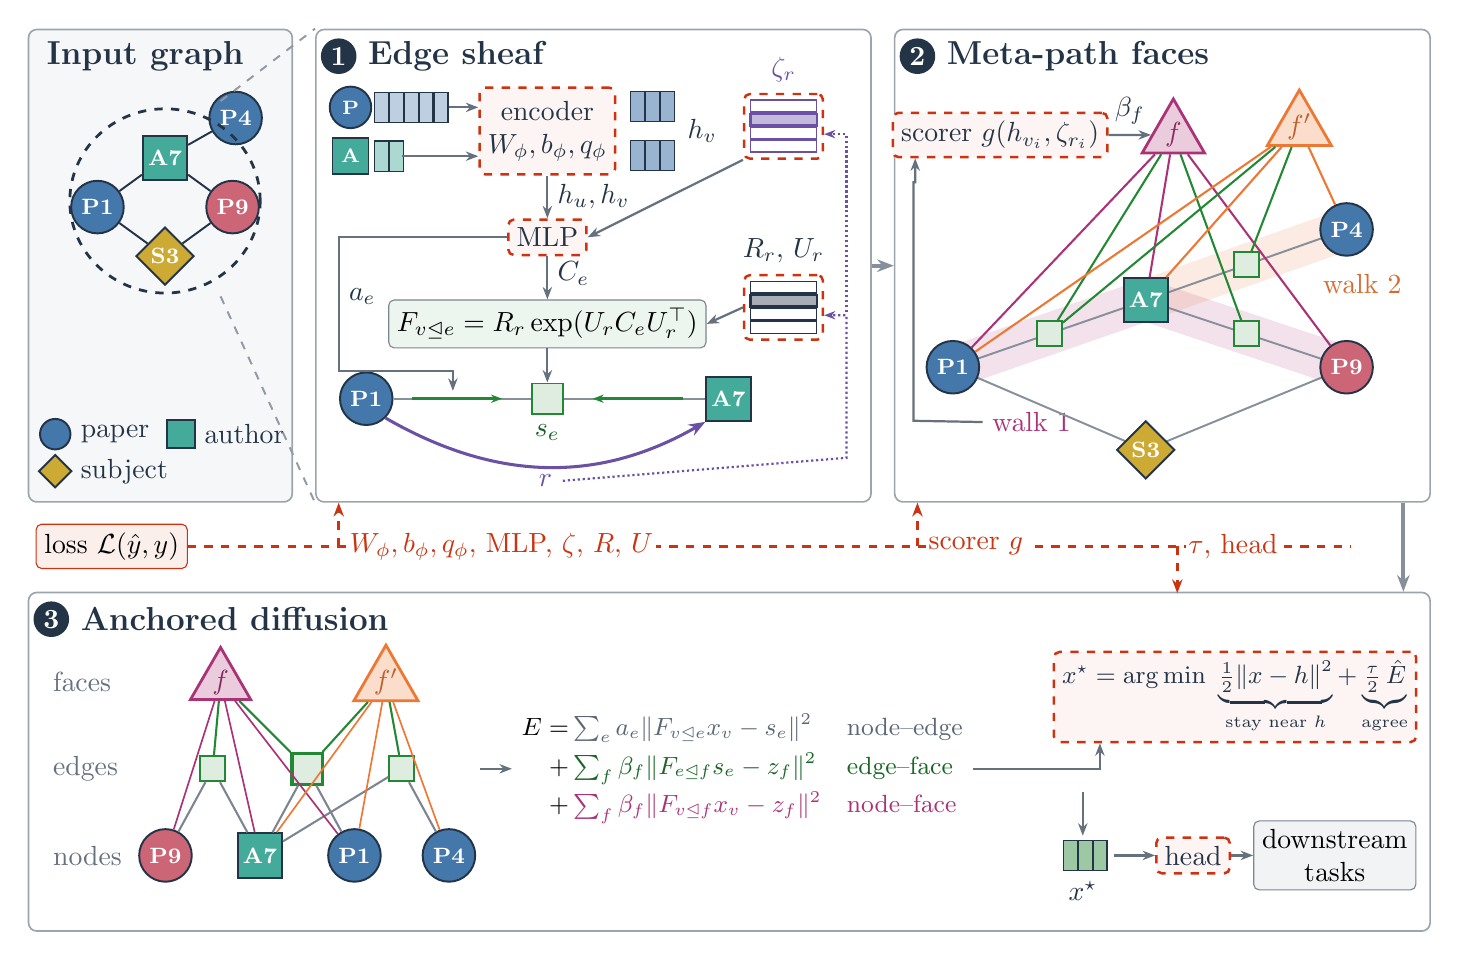
\begin{tikzpicture}
\def\WI{3.35}\def\WA{7.05}\def\WB{6.8}\def\G{0.3}\def\HA{6.0}\def\HB{4.3}\def\GR{1.15}
\pgfmathsetmacro{\xA}{\WI+\G}\pgfmathsetmacro{\xB}{\xA+\WA+\G}\pgfmathsetmacro{\Wtot}{\xB+\WB}
\pgfmathsetmacro{\yB}{-\HA-\GR}
\node[stage,minimum width=\WI cm,minimum height=\HA cm,fill=ink!4] (BI) at (0,0) {};
\node[sname] at (0.12,-0.35) {Input graph};
\node[stage,minimum width=\WA cm,minimum height=\HA cm] (B1) at (\xA,0) {};
\node[stage,minimum width=\WB cm,minimum height=\HA cm] (B2) at (\xB,0) {};
\node[stage,minimum width=\Wtot cm,minimum height=\HB cm] (B3) at (0,\yB) {};
\foreach \i/\t in {1/Edge sheaf,2/Meta-path faces,3/Anchored diffusion}{
  \node[stnum] at ($(B\i.north west)+(0.3,-0.35)$) {\i};
  \node[sname] at ($(B\i.north west)+(0.55,-0.35)$) {\t};}
% ================= input
\begin{scope}[shift={(-0.05,-0.55)},scale=0.78]
 \node[pap,fill=cA] (iP1) at (1.2,-2.2) {P1};
 \node[aut] (iA7) at (2.3,-1.4) {A7};
 \node[sub] (iS3) at (2.3,-3.0) {S3};
 \node[pap,fill=cB] (iP9) at (3.4,-2.2) {P9};
 \node[pap,fill=cA] (iP4) at (3.45,-0.75) {P4};
 \draw[ed] (iP1)--(iA7) (iA7)--(iP9) (iA7)--(iP4) (iP1)--(iS3) (iS3)--(iP9);
 \draw[ink,dashed,line width=1pt] (2.3,-2.1) ellipse (1.55 and 1.5);
\end{scope}
\node[pap,fill=cA,minimum size=11pt] at (0.35,-5.15) {}; \node[lab,anchor=west] at (0.55,-5.15) {paper};
\node[aut,minimum size=10pt] at (1.95,-5.15) {}; \node[lab,anchor=west] at (2.12,-5.15) {author};
\node[sub,minimum size=12pt] at (0.35,-5.62) {}; \node[lab,anchor=west] at (0.55,-5.62) {subject};
\draw[dashed,ink!50,line width=.7pt] (2.45,-0.92)--(B1.north west);
\draw[dashed,ink!50,line width=.7pt] (2.45,-3.4)--(B1.south west);
% ================= 1 edge sheaf
\begin{scope}[shift={(\xA,0)}]
 % type encoder
 \node[pap,fill=cA,minimum size=15pt,font=\scriptsize\bfseries] (eP) at (0.45,-1.0) {P};
 \node[aut,minimum size=13pt,font=\scriptsize\bfseries] (eA) at (0.45,-1.62) {A};
 \bars{eP}{0.2,0}{5}{cA!35} \bars{eA}{0.2,0}{2}{cAu!45}
 \node[learn,minimum height=1.1cm] (enc) at (2.95,-1.3) {encoder\\$W_{\phi},b_{\phi},q_{\phi}$};
 \draw[arr] (1.7,-1.0)--(enc.west|-0,-1.0); \draw[arr] (1.1,-1.62)--(enc.west|-0,-1.62);
 \bars{enc.east}{0.08,0.31}{3}{cA!55} \bars{enc.east}{0.08,-0.31}{3}{cA!55}
 \node[lab,anchor=west] at ($(enc.east)+(0.78,0)$) {$h_v$};
 % per-relation tables
 \ptable{zt}{5.95,-1.25}{rel}
 \node[lab,text=rel,anchor=south] at ($(zt)+(0,0.45)$) {$\zeta_r$};
 \ptable{rt}{5.95,-3.55}{ink}
 \node[lab,anchor=south] at ($(rt)+(0,0.45)$) {$R_r,\,U_r$};
 % MLP and the map
 \node[learn] (mlp) at (2.95,-2.65) {MLP};
 \draw[arr] (enc.south)--node[lab,right,pos=.5]{$h_u,h_v$}(mlp.north);
 \draw[arr] (ztbox.south west)--(mlp.east);
 \node[draw=ink!60,rounded corners=2pt,fill=grn!8,font=\normalsize,inner sep=3pt] (Fbox) at (2.95,-3.75) {$F_{v\trianglelefteq e}=R_r\exp(U_rC_eU_r^{\top})$};
 \draw[arr] (mlp.south)--node[lab,right,pos=.4]{$C_e$}(Fbox.north);
 \draw[arr] (rtbox.west)--(Fbox.east);
 % the edge
 \node[pap,fill=cA] (aP1) at (0.65,-4.7) {P1};
 \node[aut] (aA7) at (5.25,-4.7) {A7};
 \node[est,minimum size=11pt] (se) at (2.95,-4.7) {};
 \draw[nedge] (aP1)--(se)--(aA7);
 \draw[mp] ($(aP1)!0.25!(se)$)--($(aP1)!0.75!(se)$); \draw[mp] ($(aA7)!0.25!(se)$)--($(aA7)!0.75!(se)$);
 \node[lab,text=grn!70!black,anchor=north] at (se.south) {$s_e$};
 \draw[arr] (Fbox.south)--(se.north);
 \draw[arr] (mlp.west) -- (0.3,-2.65) |- node[lab,right,pos=.22]{$a_e$} (1.75,-4.35) -- (1.75,-4.6);
 \draw[-{Stealth[length=6pt]},rel,line width=1.1pt] (aP1.south east) to[out=-30,in=-150] node[pos=.5,below=-1pt,font=\normalsize,text=rel] (rr) {$r$} (aA7.south west);
 \draw[look] (rr.east) -- (6.75,-5.45) |- ($(rtbox.east)+(0,-0.1)$);
 \draw[look] (6.75,-3.6) |- ($(ztbox.east)+(0,-0.1)$);
\end{scope}
% ================= 2 meta-path faces
\begin{scope}[shift={(\xB,0)}]
 \coordinate (P1) at (0.75,-4.3); \coordinate (A7) at (3.2,-3.45); \coordinate (P9) at (5.75,-4.3);
 \coordinate (P4) at (5.75,-2.55); \coordinate (S3) at (3.2,-5.35);
 % sampled walks: faint dashed bands
 \draw[band=fcF] (P1)--(A7)--(P9);
 \draw[band=fcG] (A7)--(P4);
 \node[lab,text=fcF,anchor=north] (w1) at (1.75,-4.75) {walk 1};
 \node[lab,text=fcG!90!black,anchor=north] (w2) at (5.95,-3.0) {walk 2};
 \draw[nedge] (P1)--(A7) (A7)--(P9) (A7)--(P4) (P1)--(S3) (S3)--(P9);
 \node[pap,fill=cA] (bP1) at (P1) {P1}; \node[aut] (bA7) at (A7) {A7}; \node[pap,fill=cB] (bP9) at (P9) {P9};
 \node[pap,fill=cA] (bP4) at (P4) {P4}; \node[sub] (bS3) at (S3) {S3};
 \node[est] (q1) at ($(P1)!0.5!(A7)$) {}; \node[est] (q2) at ($(A7)!0.5!(P9)$) {}; \node[est] (q3) at ($(A7)!0.5!(P4)$) {};
 % faces
 \node[face=fcF] (F1) at (3.55,-1.35) {$f$};
 \node[face=fcG] (F2) at (5.15,-1.25) {$f'$};
 \foreach \n in {bP1,bA7,bP9} \draw[cpl=fcF] (F1)--(\n);
 \foreach \e in {q1,q2} \draw[cpl=grn] (F1)--(\e);
 \foreach \n in {bP1,bA7,bP4} \draw[cpl=fcG] (F2)--(\n);
 \foreach \e in {q1,q3} \draw[cpl=grn] (F2)--(\e);
 % scorer: reads the encodings and relation embeddings of walk 1, weights face f
 \node[learn] (gsc) at (1.35,-1.35) {scorer $g(h_{v_i},\zeta_{r_i})$};
 \draw[arr] (w1.west) -- (0.25,-4.98) -- (0.25,-1.95) -| ($(gsc.south west)+(0.3,0)$);
 \draw[arr] (gsc.east)--node[lab,above]{$\beta_f$}(F1.west);
\end{scope}
% ================= 3 anchored diffusion (bottom row, full width)
\begin{scope}[shift={(0,\yB)}]
 \node[lab,anchor=west,text=ink!70] at (0.2,-1.15) {faces};
 \node[lab,anchor=west,text=ink!70] at (0.2,-2.25) {edges};
 \node[lab,anchor=west,text=ink!70] at (0.2,-3.35) {nodes};
 \node[face=fcF,minimum size=23pt] (zf) at (2.45,-1.15) {$f$};
 \node[face=fcG,minimum size=23pt] (zg) at (4.55,-1.15) {$f'$};
 \node[pap,fill=cB] (n9) at (1.75,-3.35) {P9};
 \node[aut] (n7) at (2.95,-3.35) {A7};
 \node[pap,fill=cA] (n1) at (4.15,-3.35) {P1};
 \node[pap,fill=cA] (n4) at (5.35,-3.35) {P4};
 \node[est] (e97) at (2.35,-2.25) {}; \node[est,minimum size=11pt,line width=1.1pt] (e71) at (3.55,-2.25) {}; \node[est] (e74) at (4.75,-2.25) {};
 \draw[cpl=ink!60] (n9)--(e97) (n7)--(e97) (n7)--(e71) (n1)--(e71) (n7)--(e74) (n4)--(e74);
 \draw[cpl=grn] (zf)--(e97) (zf)--(e71) (zg)--(e71) (zg)--(e74);
 \foreach \n in {n9,n7,n1} \draw[cpl=fcF,line width=.6pt] (zf)--(\n);
 \foreach \n in {n1,n7,n4} \draw[cpl=fcG,line width=.6pt] (zg)--(\n);
 \node[font=\small,anchor=west] (eq1) at (6.15,-2.25) {$\begin{array}{@{}r@{\,}l@{\quad}l@{}}
 E= & \textcolor{ink!75}{\sum_e a_e\|F_{v\trianglelefteq e}x_v-s_e\|^2} & \textcolor{ink!75}{\text{node--edge}}\\[3pt]
 + & \textcolor{grn!75!black}{\sum_f\beta_f\|F_{e\trianglelefteq f}s_e-z_f\|^2} & \textcolor{grn!75!black}{\text{edge--face}}\\[3pt]
 + & \textcolor{fcF}{\sum_f\beta_f\|F_{v\trianglelefteq f}x_v-z_f\|^2} & \textcolor{fcF}{\text{node--face}}
 \end{array}$};
 \draw[arr] (5.75,-2.25)--(6.15,-2.25);
 \node[learn,anchor=north east,font=\small] (sol) at (17.65,-0.75) {$x^\star=\arg\min\ \underbrace{\tfrac12\|x-h\|^2}_{\text{stay near }h}+\underbrace{\tfrac{\tau}{2}\,\hat E}_{\text{agree}}$};
 \draw[arr] (eq1.east) -| ($(sol.south west)+(0.6,0)$);
 \bars{13.05,-3.35}{0,0}{3}{grn!45}
 \node[lab] at (13.4,-3.8) {$x^\star$};
 \draw[arr] (13.4,-2.55)--(13.4,-3.1);
 \node[learn] (head) at (14.8,-3.35) {head};
 \draw[arr] (13.8,-3.35)--(head.west);
 \node[draw=ink!60,rounded corners=2pt,fill=ink!6,font=\normalsize,inner sep=3pt,align=center] (ds) at (16.6,-3.35) {downstream\\tasks};
 \draw[arr] (head.east)--(ds.west);
\end{scope}
\draw[flow] (B1.east)--(B2.west);
% ================= loss band between the rows, with what each part updates
\pgfmathsetmacro{\yL}{-\HA-\GR/2}
\node[draw=lrn,fill=lrn!8,rounded corners=2pt,font=\normalsize,inner sep=3pt,anchor=west] (loss) at (0.1,\yL) {loss $\mathcal{L}(\hat y,y)$};
\draw[lrn,dashed,line width=.9pt] (loss.east)--(\Wtot-1.0,\yL);
\draw[-{Stealth[length=5pt]},lrn,dashed,line width=.9pt] (\xA+0.3,\yL)--(\xA+0.3,-\HA-0.02);
\node[font=\normalsize,text=lrn,anchor=west,fill=white,inner sep=1pt] at (\xA+0.4,\yL) {$W_\phi,b_\phi,q_\phi$, MLP, $\zeta$, $R$, $U$};
\draw[-{Stealth[length=5pt]},lrn,dashed,line width=.9pt] (\xB+0.3,\yL)--(\xB+0.3,-\HA-0.02);
\node[font=\normalsize,text=lrn,anchor=west,fill=white,inner sep=1pt] at (\xB+0.4,\yL) {scorer $g$};
\draw[-{Stealth[length=5pt]},lrn,dashed,line width=.9pt] (14.6,\yL)--(14.6,\yB-0.02);
\node[font=\normalsize,text=lrn,anchor=west,fill=white,inner sep=1pt] at (14.7,\yL) {$\tau$, head};
% flow from panel 2 to panel 3
\draw[flow] ($(B2.south east)+(-0.35,0)$) -- ++(0,-\GR+0.02);
\end{tikzpicture}
\end{document}
